%%%%%%%%%%%%%%%%%%%%%%%%%%%%%%%%%%%%%%%%%%%%%%%%%%%%%%%%%%%%%%%%%%%%%%
%%%%%%%%%  TEMPLATE IEEE PARA ENTREGA DEL ARTÍCULO FINAL DE  %%%%%%%%% 
%%%% PRÁCTICA DE INGENIERÍA ELECTRÓNICA DE LA UNIVERSIDAD CENTRAL %%%%
%%%%%%%%%%%%%%%%%%%%%%%%    BOGOTÁ, COLOMBIA    %%%%%%%%%%%%%%%%%%%%%%
%%%%%%%%%%%%%%%%%%%%%%%%%%%%%%%%%%%%%%%%%%%%%%%%%%
%%%%   AUTOR: SERGIO ANDRÉS CHAPARRO MORENO   %%%%
%%%%%%%%%%%%%%%%%%%%%%%%%%%%%%%%%%%%%%%%%%%%%%%%%%
%%%%%%%%%%%%%  VERSIÓN 1.0-ENE 2017  %%%%%%%%%%%%%
%%%%%%%%%%%%%%%%%%%%%%%%%%%%%%%%%%%%%%%%%%%%%%%%%%
\documentclass[journal]{IEEEtran}
\IEEEoverridecommandlockouts
%%%%%%%%%%%%%%%%%%%%%%%%%%%%%%%%%%%%%%
%%%%%%%% PRINCIPALES PAQUETES %%%%%%%%
%%%%%%%%%%%%%%%%%%%%%%%%%%%%%%%%%%%%%%
\usepackage{fancyhdr}
\usepackage{graphicx}
\usepackage[utf8]{inputenc}
\usepackage{color}
\usepackage{hyperref}
\usepackage{wrapfig}
\usepackage{amsmath}% http://ctan.org/pkg/amsmath
\usepackage{array}
\usepackage{multirow}
\usepackage{adjustbox}
\usepackage{amsmath}

\usepackage{algorithm}
\usepackage[noend]{algpseudocode}
\usepackage{nccmath}
%\usepackage{anysize}
\usepackage{pgfplots}
\usepgfplotslibrary{external}
\usepackage{bm}

\tikzexternalize
\usepackage{subfigure}
\usepackage{amsfonts,latexsym} % para tener disponibilidad de diversos simbolos
\usepackage{enumerate}
\usepackage{booktabs}
\usepackage{float}
\usepackage{threeparttable}
\usepackage{array,colortbl}
\usepackage{ifpdf}
\usepackage{rotating}
\usepackage{cite}
\usepackage{stfloats}
\usepackage{url}

\usepackage{listings}
\usepackage{color}

\lstset{
  basicstyle=\ttfamily,
  columns=fullflexible,
  frame=single,
  breaklines=true,
  postbreak=\mbox{\textcolor{red}{$\hookrightarrow$}\space},
}

\newcolumntype{P}[1]{>{\centering\arraybackslash}p{#1}} 
\newcommand{\tabitem}{~~\llap{\textbullet}~~}
\newcommand{\ctt}{\centering\scriptsize\textbf} %%\ctt abrevia el comando \centering\scriptsize\textbf
\newcommand{\dtt}{\scriptsize\textbf} 
\renewcommand\IEEEkeywordsname{Palabras clave}


% correct bad hyphenation here
\hyphenation{op-tical net-works semi-conduc-tor} 

\graphicspath{ {Figs/} } 



\newcommand{\MYhead}{\smash{\scriptsize
\hfil\parbox[t][\height][t]{\textwidth}{\centering
\begin{picture}(0,0) \put(-0,-15){
\includegraphics[width=30mm]{cued}} \end{picture} \hspace{6.5cm}
University of Cambridge \hspace{5.3cm} Version 1.0\\
\hspace{6.6cm} Department of Engineering \hspace{5cm} Date 08/02/19\\
\underline{\hspace{ \textwidth}}}\hfil\hbox{}}}
\makeatletter
% normal pages
\def\ps@headings{%
\def\@oddhead{\MYhead}%
\def\@evenhead{\MYhead}}%
% title page
\def\ps@IEEEtitlepagestyle{%
\def\@oddhead{\MYhead}%
\def\@evenhead{\MYhead}}%
\makeatother
% make changes take effect
\pagestyle{headings}
% adjust as needed
\addtolength{\footskip}{0\baselineskip}
\addtolength{\textheight}{-1\baselineskip}
\usepackage{nomencl}
\makenomenclature
\pgfplotsset{compat=1.9}

\makeatletter
\def\BState{\State\hskip-\ALG@thistlm}
\makeatother


\begin{document}

\title{3G3 Coursework: Coding In Visual Cortex}

\author{Tom Xiaoding Lu\\
				\textit{xl402@cam.ac.uk}\\
				Pembroke College\\% stops a space
} %\thanks anexa una nota a pie de página donde se puede colocar alguna información sobre la naturaleza del documento.
%%%%%%%%%%%%%%%%%%%%%%%%%%%
%\thanks{El presente documento corresponde al articulo final del proyecto de práctica de ingeniería electrónica 3 presentado en la Universidad Central durante el periodo 2017-1.}
% Comando que indica la generación del título
\maketitle

\begin{abstract}
This coursework investigates two visual image coding mechanisms, the \textit{compact coding} and the \textit{spare distributed coding} mechanisms. Through image reconstruction using the basis generated by these two mechanisms, the underlying principles involved in sensory information processing used in the visual cortex can be uncovered. \end{abstract}

\section{Introduction \& Background Information}
The visual system can exploit the structure of natural images' state space, and use efficient coding schemes to achieve image encoding and reconstruction.\\
Consider the state-space of a receptor array such as the photoreceptors in the retina, modelling the receptive field as an array composed of $N$ receptors, each of which can represent any value within a range of luminance, each image can then be represented as a single point in such high dimensional array. Although the number of possible images that can be represented is vast, typical (natural) images do not span the entire state space. \\
By taking adjacent pixels at random locations in natural images and plotting their intensities against each other, figure \ref{fig:a} and figure \ref{fig:b} show the correlation between neighbouring pixels of random and structured images respectively. \\
\begin{figure}[htbp]
\centering     %%% not \center
\subfigure[random images]{\label{fig:a}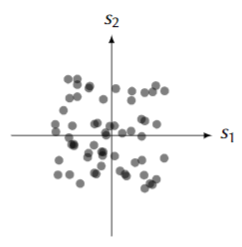
\includegraphics[width=40mm]{s1.PNG}}
\subfigure[structured images]{\label{fig:b}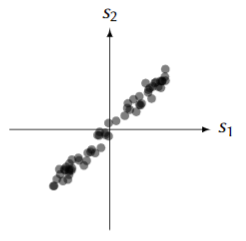
\includegraphics[width=40mm]{s2.PNG}}
\caption{Correlation between neighbouring pixels}
\end{figure}
Clearly, for structured images, there is a linear, positive correlation between neighbouring pixels, as the structured (natural) images mainly consist of blocks of colours and colour gradients; edges which result in sharp discrepancies between neighbouring pixels are rare. \\
As natural images are highly structured, the visual system can exploit such structures through efficient coding mechanisms. Two possibilities, \textit{Compact coding} and \textit{Sparse distributed coding} are investigated and are illustrated in figure \ref{fig:3}.

\begin{figure}[htbp]
\centering     %%% not \center
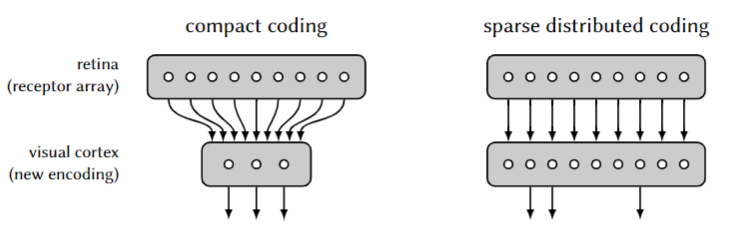
\includegraphics[width=90mm]{s3.PNG}
\caption{Two different forms of coding the retinal receptor array to activity in visual cortex}
\label{fig:3}
\end{figure}
 The \textit{Compact coding} scheme proposes using minimal number of neurons to encode the output of the retinal receptors. The \textit{Sparse distributed coding} scheme aims to decrease the average activity of neurons in encoding the retinal receptors output.\\
 The aim of the coursework is to compare the retinal receptive field representation through the two coding schemes with the receptive field of a neuron in V1 obtained experimentally. Simple cells in V1 have receptive fields with the following characteristics:
 \begin{enumerate}
     \item Localized within a small region of retinal space
     \item Respond best to a bar of light at a particular position, orientation and width
 \end{enumerate}
The responses of simple cells to light can be computed from convolving the retinal image with the two-dimensional filters shown in figure \ref{fig:simple_cells}, which are the filters the theoretical model aims to produce.
\begin{figure}[htbp]
\centering     %%% not \center
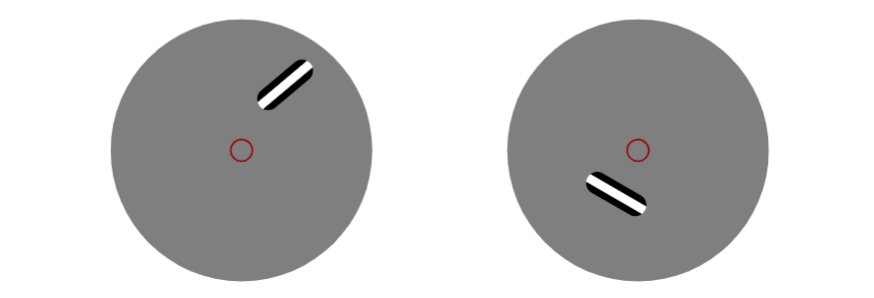
\includegraphics[width=80mm]{s4.PNG}
\caption{The receptive fields of two typical simple cells in V1, acting as linear filters}
\label{fig:simple_cells}
\end{figure}

\section{Image Reconstruction From Image Bases}
We assume that a given retinal image in visual space can be reconstructed through a \textbf{linear combination} of basis functions given by V1 neuron receptive fields. The weights can be seen as the activations of the corresponding V1 neurons. \\
Given an image $S(x,y)$, the neural population output which approximates the image is denoted $\hat{S}(x,y)$. This output is constructed through the superposition of a set of neurons, each $ith$ neuron contributes a basis function $\phi_i(x,y)$, with its activation denoted as $a_i$. Equation \ref{eq:image} encapsulates the relationship between individual neuron's response and neural population output (approximated image).

\begin{equation}
    \hat{S}(x,y) = \sum_i a_i \phi_i (x,y)
    \label{eq:image}
\end{equation}
\subsection{Compact Coding}
Principal Component Analysis (PCA) is a dimensionality reduction technique, used to find a reduced set of orthogonal vectors that encapsulate the directions of maximum variance of the original retinal state space. These vectors can be used as basis functions used to achieve compact coding.
\begin{figure}[htbp]
\centering     %%% not \center
\subfigure[Natural images]{\label{fig:pca1}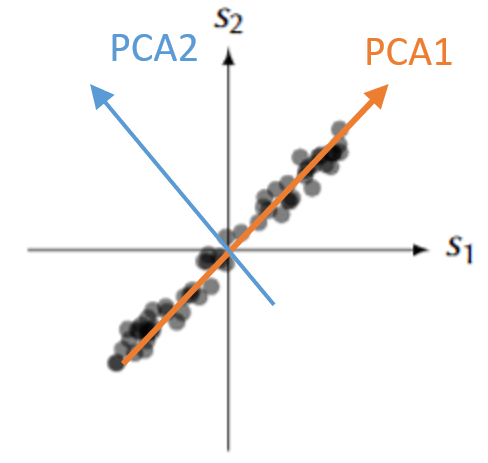
\includegraphics[width=40mm]{c1.PNG}}
\subfigure[Lossless PCA1 images]{\label{fig:pcai}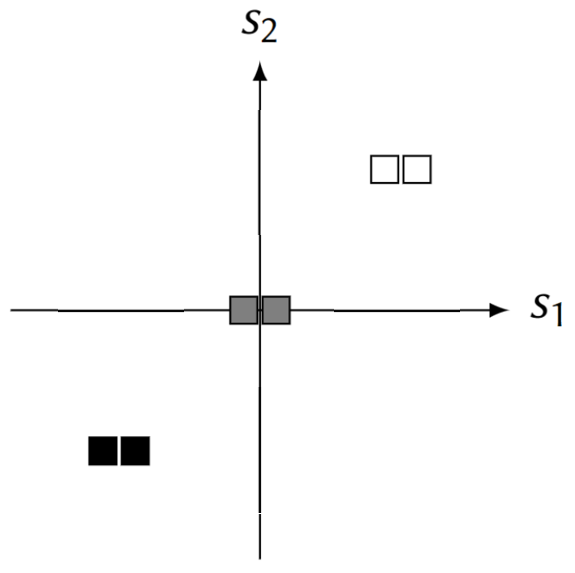
\includegraphics[width=40mm]{c4.PNG}}

\subfigure[Dataset A]{\label{fig:pca2}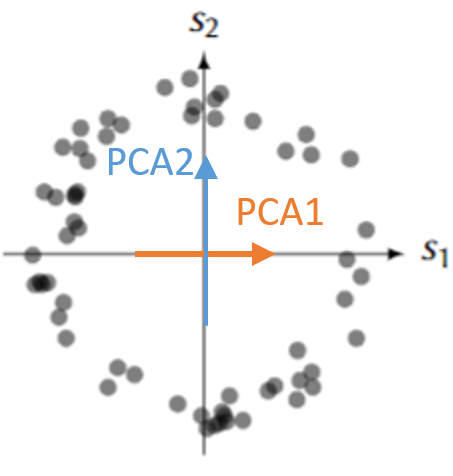
\includegraphics[width=40mm]{c2.PNG}}
\subfigure[Dataset B]{\label{fig:pca3}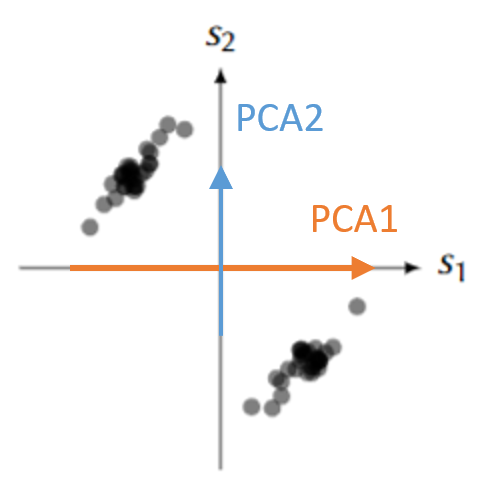
\includegraphics[width=40mm]{c3.PNG}}
\caption{Principal components of different datasets}
\end{figure}
In the simplified example of two-pixel natural images shown in figure \ref{fig:pca1}, the axis along the positive diagonal is the first principal component vector as it is the most informative direction. Assuming it also represents the distribution of natural 2-pixel images, figure \ref{fig:pcai} represents examples of 2-pixel images that could be represented without error using only PCA1.\\
PCA has limitations; in figure \ref{fig:pca2} and \ref{fig:pca3},  when a given data set is not linearly distributed but might be arranged along with non-orthogonal axes or well described by a geometric parameter, PCA could fail to represent and recover original data from projected variables. In these cases, feature transformation is required to map the data onto other dimensions.\\
\begin{figure}[htbp]
\centering     %%% not \center
\subfigure[I1: Text image]{\label{fig:ex1}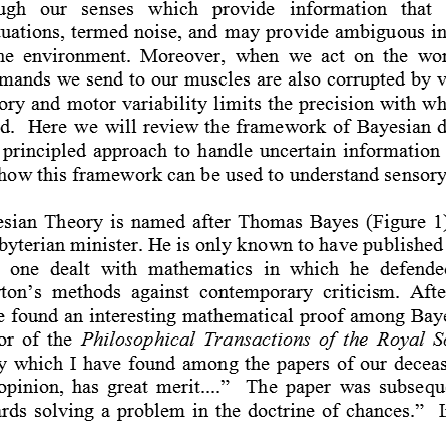
\includegraphics[width=33mm]{i1.PNG}}
\subfigure[I2: Natural scene]{\label{fig:ex2}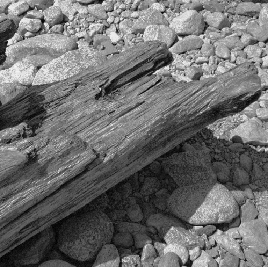
\includegraphics[width=32mm]{i2.PNG}} 
\subfigure[I2w: Natural scene gradient]{\label{fig:ex2w}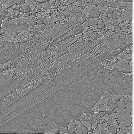
\includegraphics[width=32mm]{i2w.PNG}}
\subfigure[I3: White noise]{\label{fig:ex3}
\includegraphics[width=33mm]{i4.PNG}}
\caption{Samples from training images}
\end{figure}
In order to test the different coding mechanisms, different image sets are created as training data for forming basis functions. Figure \ref{fig:ex1} and figure \ref{fig:ex2} are natural images of text and natural scene respectively. Images from I2w set, with an example shown in figure \ref{fig:ex2w} are the gradient of the I2 images. Images in I3 are generated white noise, used to further validate the coding schemes.\\
By performing PCA on the image sets I1, I2 and I3, their major principal components and the amount of variance that each basis function accounts for on a log-log scale are shown in figure \ref{fig:pca_cov}. The minimum number of principal components needed to account for over 90\% of total variance is 102, 12, 206 respectively for the three image sets. This result should not be surprising as natural scenes in I2 are most structured, text image in I1 is also structured, however, characters have finer defining features than natural images. The images in I3 are generated noise which is unstructured, hence PCA is unable to reduce the dimensions of the image space. \\
\begin{figure}[]
\centering     %%% not \center
\subfigure[I1 basis]{\label{fig:i1_basis}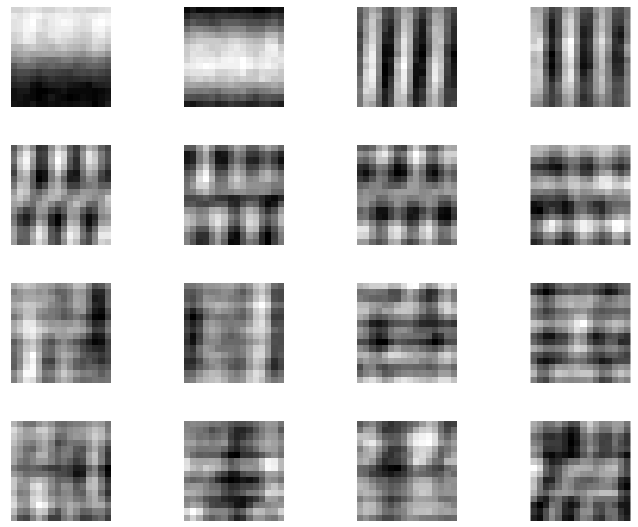
\includegraphics[width=40mm]{pca_I1.png}}
\subfigure[I1 basis variance coverage]{\label{fig:i1_cov}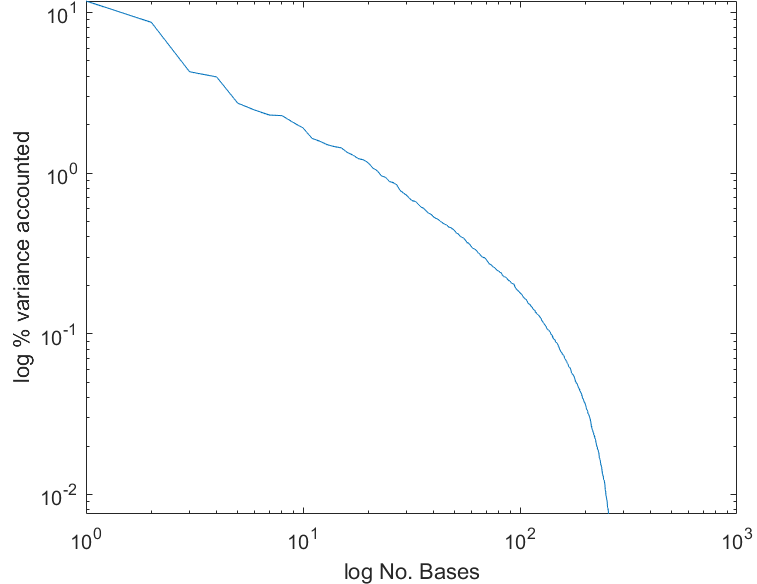
\includegraphics[width=43mm]{loglog.png}}

\subfigure[I2 basis]{\label{fig:i2_basis}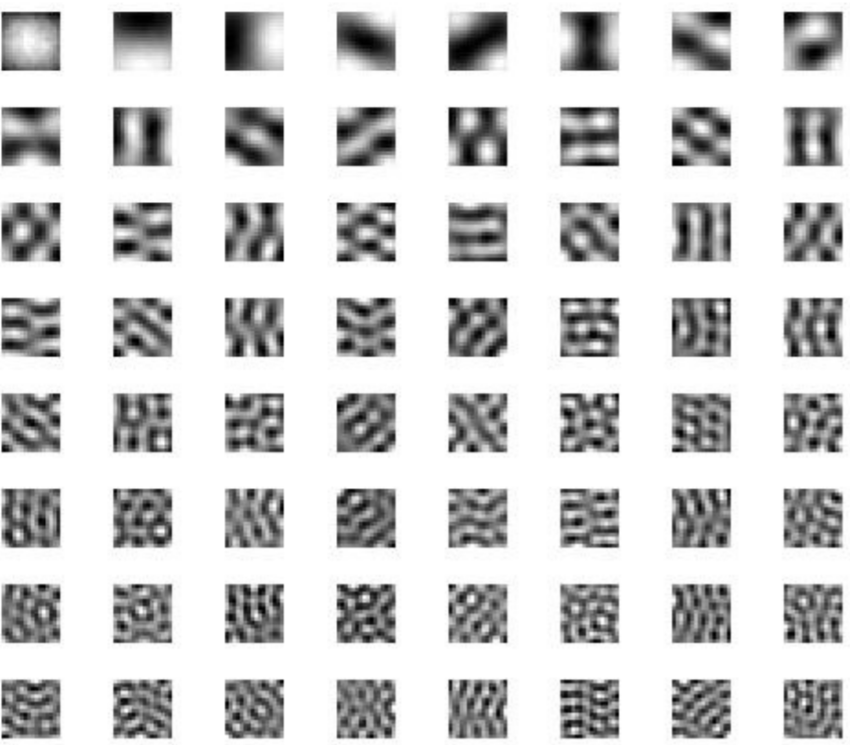
\includegraphics[width=40mm]{i2_bases.png}}
\subfigure[I2 basis variance coverage]{\label{fig:i2_cov}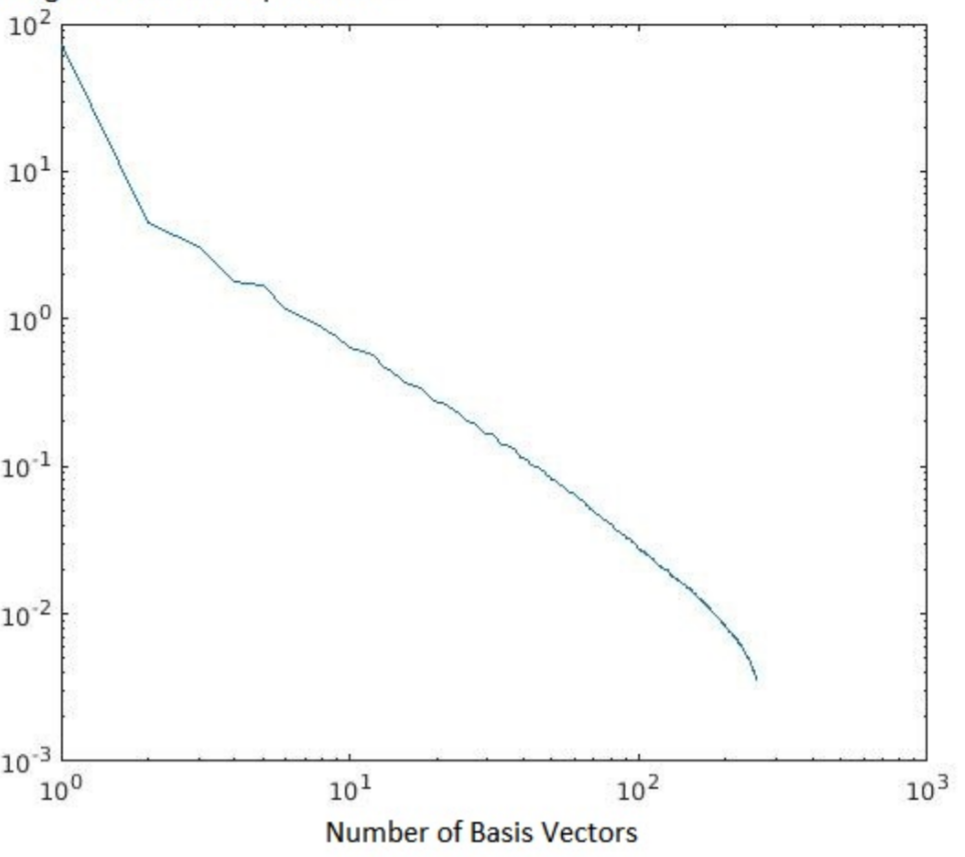
\includegraphics[width=43mm]{loglog_3.PNG}}
\subfigure[I3 basis]{\label{fig:i3_basis}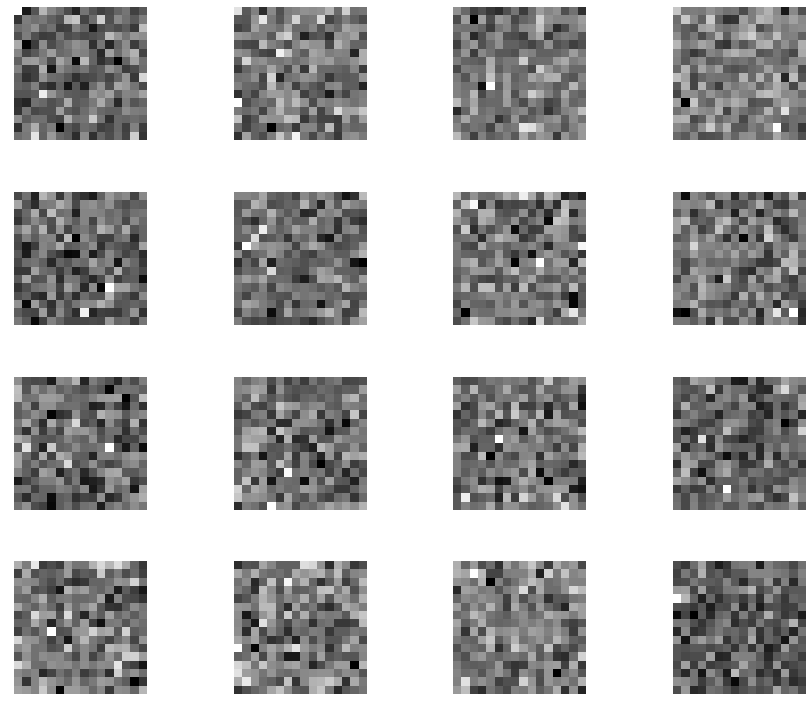
\includegraphics[width=40mm]{i3_bases.png}}
\subfigure[I3 basis variance coverage]{\label{fig:i3_cov}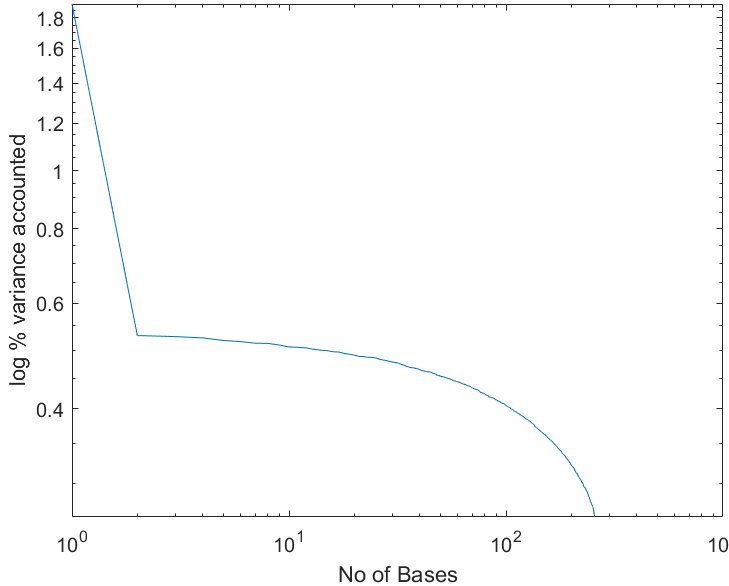
\includegraphics[width=43mm]{loglog_2.png}}
\caption{PCA basis functions and coverage for different image sets}
\label{fig:pca_cov}
\end{figure}
To investigate the image features which the basis functions extract through PCA, the example images are convolved with the top three basis functions accounting for most amount variance. Figure \ref{fig:covs} shows the top three basis functions (kernels) for I1. The text image, figure \ref{fig:ov1} shows a horizontal gap extraction kernel, responsible for detecting gaps between lines. Figure \ref{fig:ov2} shows a kernel which responses to the lines of texts themselves. Figure \ref{fig:ov3} shows a kernel which responses to gaps between characters. Intuitively, the basic structure of passages from a corpus consist of mainly these three features, gaps between lines, lines of texts and gaps between characters. \\
Similarly, for I2 natural images set, figure \ref{fig:covs2} shows that the first basis function is a low pass filter, extracting the smoothed image. The second and third basis functions extract horizontal and vertical edges of the image respectively. The higher order basis functions become more complicated and each account for less variance.\\
PCA decomposition deconstructs input images into a linear combination of basis functions which can be seen as basic image features. It is seen that through performing PCA on natural images, the most important basis function shown in figure \ref{fig:ov4} matches with the simple cells' receptive fields from the Lateral Geniculate Nucleus (LGN), which provide on-centre-off surround responses. However, simple cells' responses from the V1-cortex is not simulated by higher-order basis functions, therefore compact coding through PCA is likely not to be a good model for modelling receptive fields from the visual cortex.

\begin{figure}[]
\centering     %%% not \center
\subfigure[]{\label{fig:ov1}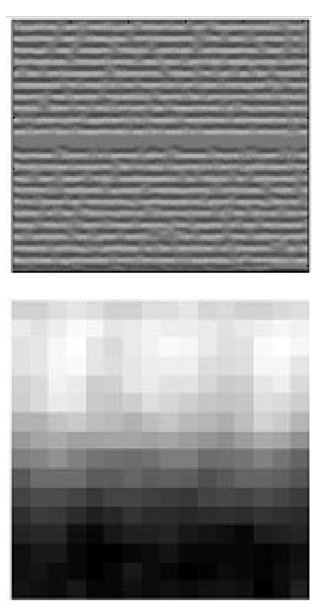
\includegraphics[width=26.3mm]{ov_1.PNG}}
\subfigure[]{\label{fig:ov2}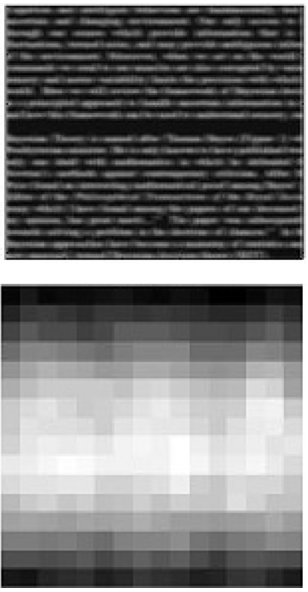
\includegraphics[width=26mm]{ov_2.PNG}}
\subfigure[]{\label{fig:ov3}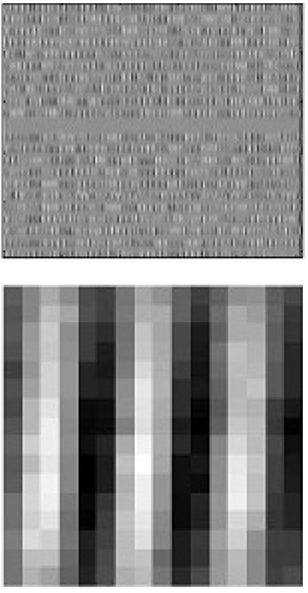
\includegraphics[width=26mm]{ov_3.PNG}}
\caption{I1 convolved images and their corresponding features}
\label{fig:covs}
\end{figure}

\begin{figure}[]
\centering     %%% not \center
\subfigure[]{\label{fig:ov4}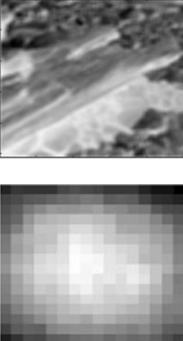
\includegraphics[width=25.5mm]{ov_4.PNG}}
\subfigure[]{\label{fig:ov5}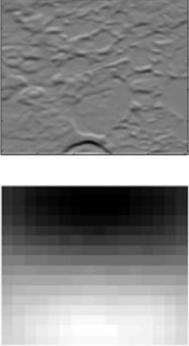
\includegraphics[width=26mm]{ov_5.PNG}}
\subfigure[]{\label{fig:ov6}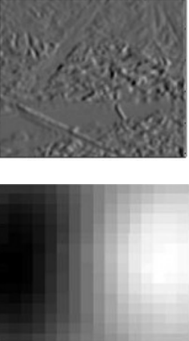
\includegraphics[width=26.4mm]{ov_6.PNG}}
\caption{I2 convolved images and their corresponding features}
\label{fig:covs2}
\end{figure}

\subsection{Sparse Distributed Coding}
If PCA used in compact coding is seen as a solution to an optimization problem, its complicated higher order basis functions can be seen as overfitting solutions. In sparse distributed coding, we introduce a regularization term which aims to reduce the total amount of activation (weights) used when reconstruction the retinal space from basis functions. This regularization can also be seen as a prior from the Bayesian perspective. From equation \ref{eq:image}, sparse distributed coding's cost function can be written as:
\begin{eqnarray}
\mathcal{C}(\{\phi_i\},\{a_i\}) &=& \sum_{x,y}[S(x,y) - \hat{S}(x,y)]^2 + \lambda \sum_i H (a_i)\label{eq:cost}
\\
&=& (\bm{s}-\bm{Ba})^T(\bm{s}-\bm{Ba}) + \lambda \sum_i H(a_i)
\label{eq:cost1}
\end{eqnarray}
Where $H(a_i) = \log (1+ \dfrac{a_i^2}{\sigma^2})$ chosen as the regularization term as it is smooth (differentiable) and monotonically increasing. To speed up computation time, equation \ref{eq:cost} is vectorized, the matrix $\bm{B}$ has row vectors as basis functions and vector $\bm{a}$ stores all activations for different basis functions.\\
The cost function is nonlinear because $H(a_i)$ is nonlinear, standard gradient descent techniques can be used to minimize the cost function with respect to both basis function matrix $\bm{B}$ and activations $\bm{a}$:
\begin{eqnarray}
\dfrac{\partial{\mathcal{C}}}{\partial\bm{a}} &=& s \bm{B^T Ba} - 2 \bm{B^T s} + 2\lambda \dfrac{\bm{a}}{\sigma^2 + \bm{a}^2}\label{eq:grad1}\\
\dfrac{\partial{\mathcal{C}}}{\partial\bm{B}} &=& 2\bm{Baa^T} - 2\bm{sa^T}\label{eq:grad2}
\end{eqnarray}
After calculating the gradients, the gradient descent algorithm can be implemented through: \begin{enumerate}
    \item Starting with a random set of basis functions (randomized $\bm{B}$ matrix).
    \item Given this set of fixed basis functions, find the set of activations which minimizes the cost $\mathcal{C}$ using equation \ref{eq:grad1}.
    \item Update the basis functions through minimizing $\mathcal{C}$ using equation \ref{eq:grad2}
\end{enumerate}
The gradient descent method is implemented in MATLAB. Using library function \textit{minimize()}, optimizing the parameters over 500 iterations took 0.756 seconds, which is slow due to MATLAB's Just-In-Time compilation. The conjugate gradient descent method implemented in C is used instead; optimization over 500 iterations took 2.63 $ms$, which is two magnitudes faster. 
\subsection{Stochastic Gradient Descent and Batch Normalization}
Stochastic gradient descent is implemented in order to minimize the cost function in batches. At each time step, subimages are extracted by sampling the training image set at random, and the gradient descent algorithm is used to update $\bm{B}$ and $\bm{a}$.\\ Without batch normalization, the values in the basis functions would tend to grow without bound due to gradient explosion, as an early on large activation causes a large output response from the neuron (basis function), which cascades through each training step. This problem can be solved by re-scaling the magnitude of each basis function after each time step. The re-scaling factor for each basis function is proportional to the amount required to stretch its activation to some arbitrary target activation. This way we constrain the activations after each batch to be centered around some target activation so the problem of exploding gradient is solved. This way higher learning rates can also be afforded as batch normalization also reduces dependence on parameter scale. \\
By finding the basis functions using the sparse code mechanism, over training datasets I3 and I2w, figure \ref{fig:spar} shows the 64 extracted basis functions. For the dataset I3, it is observed that the basis functions extracted are very different from PCA basis functions, they are either only responsive to a single pixel in a subimage or responsive to all but one pixel in a subimage. This suggests that I3 was generated artificially to have uniformly distributed random high intensity pixels on a background of low intensity pixels. The I3 basis functions also validate the performance of the sparse code mechanism, as the way to represent a typical I3 image with minimum number of neurons is to have one neuron responsible for one pixel in the subimage. \\
Finally, basis functions are extracted from natural images using the 'sphered' version of I2, in which variances in different directions have been equalized (this is seen as a input features normalization). Comparing these basis functions to the simple cell model shown in figure \ref{fig:simple_cells}, we can see that these basis functions are very representative of the simple cells' receptive fields. They are responsive towards specific gradients at specific locations, which can be characterized as being localized, oriented and bandpass.
\begin{figure}[htpb]
\centering     %%% not \center
\subfigure[I3 noise image set]{\label{fig:spar_2}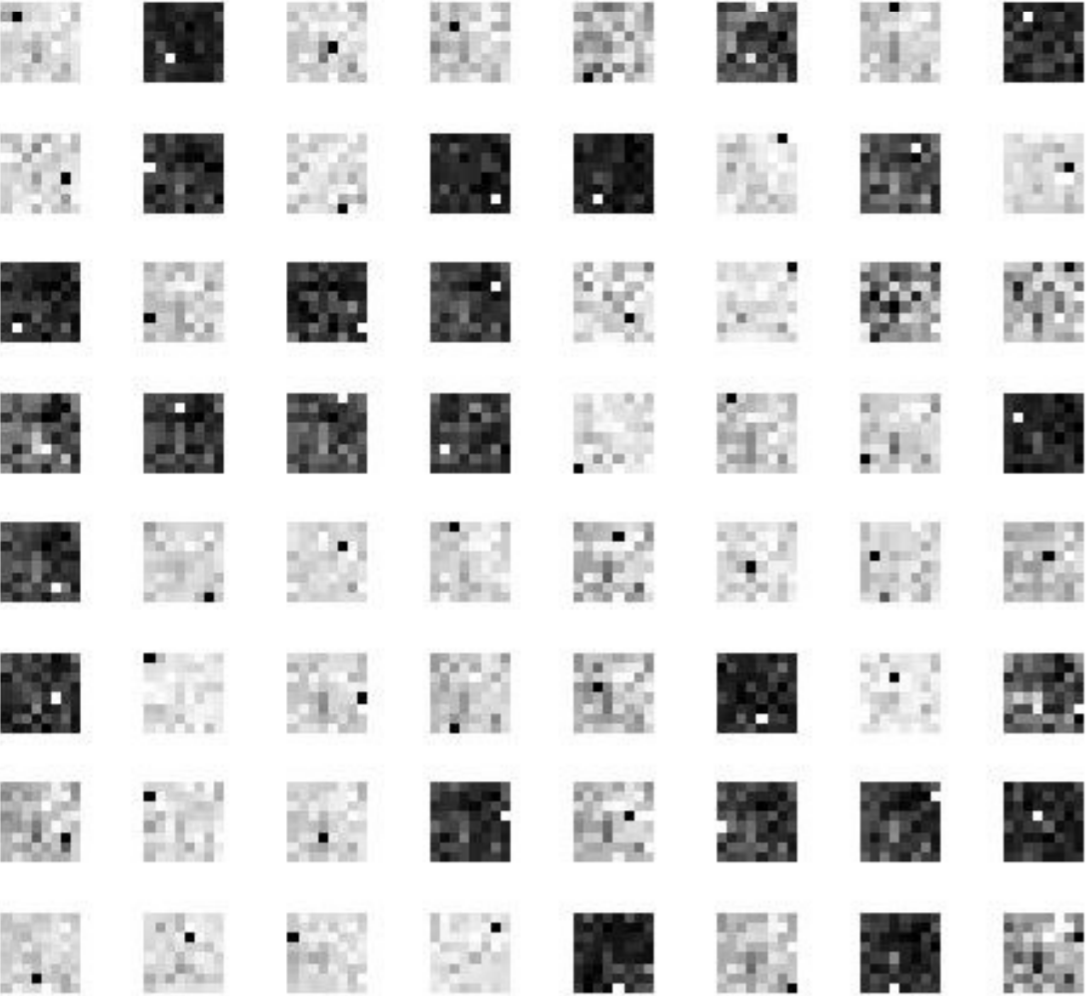
\includegraphics[width=80mm]{spar_2.PNG}}
\caption{Spars code basis functions}
\subfigure[I2w natural image set]{\label{fig:spar_1}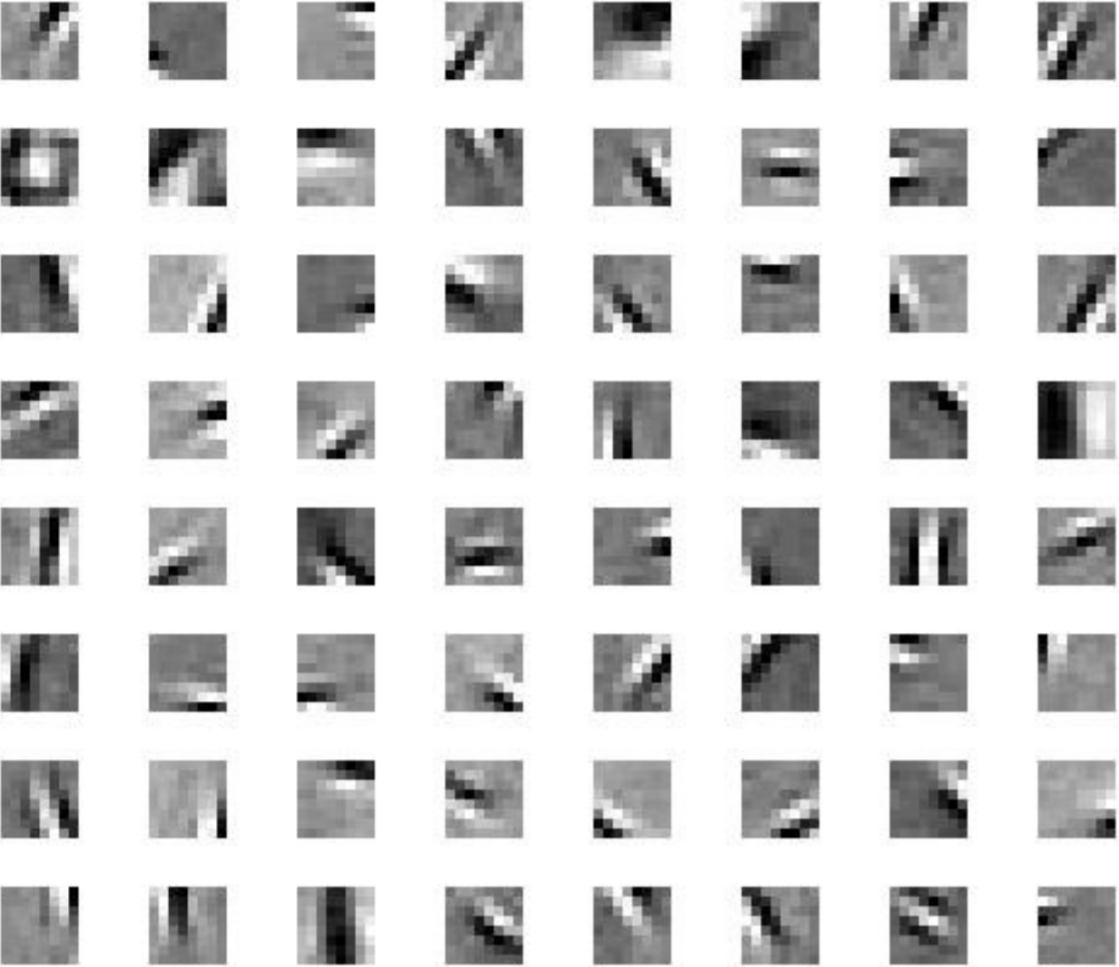
\includegraphics[width=80mm]{spar_1.PNG}}
\label{fig:spar}
\end{figure}
\section{Conclusions}
This coursework aims to predict the receptive field of simple cells through compact coding and sparse coding mechanisms. Through comparing model output with results from neurobiological experiments, we can confirm that compact coding through PCA is a simple way of approximating the receptive field, however, its higher-order basis functions are not representative. Sparse coding is the most likely model to be adapted by the visual cortex as it produces basis functions with similar responses compared with the simple cells, which are localized, oriented and bandpass. The neuroiological implications of sparse coding is not discussed within the coursework. Possible explanations involve better signal to noise ratio, energy efficiency and feature detection which assists recognition in later stages of the visual cortex. \\
The activation regularization function $H(a_i)$ in equation \ref{eq:cost} is chosen without explanations. Further experiments can focus on the effects of using different regularization functions. Our model also assumes that the activations from individual neurons are reliable and noiseless, whereas in reality neural outputs are noisy. The unreliable activations can be accounted for in future experiments and coding strategies can expand upon sparse coding to achieve more representative coding strategy by the visual cortex.

\section{Appendix: Selections of MATLAB Code}
\subsection{Sparse Code cost and activation gradient}
\begin{lstlisting}[language=MATLAB]
function [cost,dcost]=spfunc(a,B,s,sigma,lambda)
%s is the subimage vector
%B is the base matrix
%a is the activations
% cost is the cost
% dcost is the vector of the derivatives of the cost with respect to the
% activations
cost= (s-B*a)' * (s-B*a) + lambda * sum(log(1 + a.^2/sigma^2));
dcost= 2*(B'*B)*a - 2*B'*s + 2*lambda * a ./ (a.^2 + sigma^2);
\end{lstlisting}
\subsection{Sparse Code basis function gradients}
\begin{lstlisting}[language=MATLAB]
function dcost=basefunc(a,B,s)
%s is the subimage vector
%B is the base matrix
%a is the activity vector
% dcost is the returned vector of the partial derivatives 
% of the cost with respect to the bases
% you should calculate dcost here 

dcost= 2* B * (a* a') - 2*s*a';
\end{lstlisting}
\end{document}




















